

\documentclass[10pt]{report}

\usepackage{geometry}
\geometry{
  a4paper,
  textwidth=7cm,
  left=40mm,
  right=25mm,
  top=25mm,
  bottom=25mm,
  }
\usepackage[utf8]{inputenc}
\usepackage{cite}
\usepackage{url}
\usepackage{dsfont}
\usepackage[T1]{fontenc}
\usepackage{graphicx}
\graphicspath{{images/}}
\usepackage{mathtools}
\usepackage{amsmath}
\usepackage{subcaption}
\setlength{\parindent}{0em}
\setlength{\parskip}{1em}
\usepackage{csquotes}
\setcounter{secnumdepth}{3}
\usepackage[ruled]{algorithm2e}
\usepackage{algorithmic}


%
% Diagrams tool.
%
\usepackage{tikz}
\usetikzlibrary{mindmap,trees,matrix,shapes.multipart,shapes.geometric,fit,scopes,shapes.misc,shadows}
\tikzset{
  >= latex,
  el/.style={ellipse, draw, text width=8em, align=center},
  rs/.style={rectangle split, draw, rectangle split parts=#1},
  ou/.style={draw, inner xsep=1em, inner ysep=1ex, fit=#1},
  cy/.style={cylinder, shape border rotate=90, draw,minimum height=3cm,minimum width=2cm}
}
%
% End Tikz Did
%

\usepackage{chngcntr}
\counterwithout{figure}{chapter}
\counterwithout{table}{chapter}
\usepackage{caption}
\captionsetup[figure]{font=footnotesize,labelfont=footnotesize}

\usepackage{titlesec}
\titleformat{\chapter}[display]
{\normalfont\huge\bfseries}{\chaptertitlename\ \thechapter}{20pt}{\Huge}   
\titlespacing*{\chapter}{0pt}{-50pt}{25pt}
\titlespacing*{\section}{0pt}{0pt}{0pt}
\titlespacing*{\subsection}{0pt}{0pt}{0pt}
\title{Analysing Narratives: Automatic Descriptive Feature Extraction Through Latent Entity modelling}
\author{Adam Slack}
\date{}

\begin{document}
 
\begin{titlepage}
  \maketitle
\end{titlepage}

\addcontentsline{toc}{section}{Declaration}
\section*{Declaration}
I declare that this work is my own and not someone elses. May god beat down upon me with hellfire should this declaration be falsly claimed.


\newpage
\addcontentsline{toc}{section}{Abstract}
\section*{Abstract}
Latent Entities are approximations of entities found within a corpus allowing for similar entities to be grouped into classes. Through the use of a document segmentation method processing entities and associated terms, LDA can be applied with the intention of extracting topics from each entity segmentation.



% TABLE OF CONTENTS - SPACING CHANGE, TOC, SPACING CHANGE
\renewcommand{\baselinestretch}{0.5}\normalsize
\tableofcontents
\listoffigures
\listoftables
\renewcommand{\baselinestretch}{2.0}\normalsize

%
%
% Chapter 1 - Introduction
%
%
\chapter{Introduction}

\section{Introduction}
The Web; A seemingly ever-expanding resource, with data being generated and information published at an accelerating rate~\cite{WebServer-lc}. As more gain access to the internet, the rate at which new information is made available will only increase. Whether the origins of data be, social media, news outlets, or e-commerce reviews, much of the resources on the web exist in a natural language format. From this data there exists underlying information that can be extracted and utilised in decision making process. Given the amount of processing required to consume data on this scale, it is necessary to ensure that computational methods exist that can accommodate for individual or business needs to understand data. Many methods for Methods that allow the processing of data to extract surface level information exist, however there is room for further understanding. By relating distinct pieces of information or subsets of data, it is possible to frame or contextualise a solution to a problem within a wider setting. This paper aims to provide a novel method capable of providing succinct summaries of documents in terms of entity topics.

Information Retrieval (IR), Machine Learning (ML), and Natural Language Processing (NLP) when considered in conjunction with each other,  concern themselves with the extracting of information from data in a natural language texts. Relating textual data yields information valuable to many different entities, including businesses when marketing products, individuals when choosing what to read, and even researchers considering the current state of a research area. For a business, relating entities extracted from texts, can help identify target groups to aim products at. For an individual, relating entities can assist in decisions on what to read, buy, and watch based on similarities between things that they do and don’t like. For research, the identification of common themes, or prominent authors can be achieved through the relating of entities.

A Latent Entity in this investigation is defined as an abstract representation of some entity that can be used to describe one or more concrete entities. Thus the term Latent Entity Modelling is defined as a transformation from a corpus of text to a collection of Latent Entities describing a corpus. Latent Entities represent a layer of abstraction from a corpus,  wherein it is possible to describe the corpus as a whole in terms of the Latent Entities.

Entity models build upon the concept of topic modelling, particularly the kinds of topics derived through Latent Dirichlet Allocation. A Topic in this sense is a probability distribution of words, such that the degree of membership for each word in a topic indicates the probability of that word being an indicator of that topic. By performing clustering on entities expressed interms of entity topic models, this paper investigates if it is possible to 


\section{Aims and Objectives}
The aims of this project are two-fold. The first aim is to utilise and extend natural language processing methods to model and extract latent information describing entities within narratives. The second aim is to develop a system within which corpora can be easily and effectively analysed and explored when methods developed for aim one are applied.

Natural Language Processing is a large field with many analytical methods available for modelling purposes, and as such the scope of the first aim is required to be well defined. Objectives for the first aim include:

\renewcommand{\baselinestretch}{1.0}\normalsize
\begin{itemize}
\item To survey the fields of Natural Language Processing and Topic Modelling to identify methods valuable for the task of Entity-Topic Modelling.
\item To Define a Entity-Topic Modelling method capable of deriving interpret-able topics which describe entities within narratives.
\end{itemize}

The second aim involves the development of a software environment, the objectives of which include:
\begin{itemize}
\item To develop a front-end user interface for the visual exploration of entity-topic models.  
\item To implement back-end infrastructure allowing for dynamic visualisations in front-end user interfaces.
  \item To create a software pipeline that extracts entity-topic data from a provided corpus.
\end{itemize}
\renewcommand{\baselinestretch}{2.0}\normalsize

\section{Motivation}
Motivations for this project include the need for more effective methods and tools capable of analysing data in natural language form. Additionally the development of tools utilising these methods can assist in providing others with means of understanding more about themselves, their habits, and their preferences.


%
%
%  Chapter 2 - Literature Review
%
%
\chapter{Literature Review}

\section{Introduction}
Natural Language Processing (NLP) is a vast field of study within Computer Science and Computational Intelligence, the focus of which is the development of intelligent systems capable of handling data in the form of natural language. The task of extracting Latent Entity Models is one that will touch upon many areas of NLP, including Part-of-Speech (POS) tagging, Named Entity Recognition (NER), and Latent Topic Modelling. Given that the focus of this paper is the extraction of descriptive information of narratives, it is necessary to consider the field of Information Retrieval and existing methods of descriptive summarisation as well.

It is possible to divide NLP into two large schools of thought; One involves the processing of natural language such that machine usable resources are available, the other is concerned with the application of information resulting from processed natural language. Whilst many NLP tasks require methods for parsing, understanding, or synthesising spoken words, this paper is only considering written texts. As such, the spoken language aspects of NLP will be overlooked.

Parsing written texts begins with tokenization. This is the division of a single string of characters in to strings representing sentences or words. Often text is tokenized into sentences, and each sentence is then tokenized into words. Once a text is expressed with basic sentence and word structure it is possible to apply additional processing steps. POS tagging is the application of tags to sequences of words, each tag and resulting sequence represents the grammatical structure of a sequence of words. NER is the extraction of entities from natural language, entities are tagged depending on their type. NER is performed after tokenization, however it doesn’t necessarily rely on text being POS tagged first.

There are a range of NLP tasks involving the applications of natural language parsing. From Customer relation Chatbots, to Document Summarisation and Relation. Whilst many applications involve the use of parsed text features, many also orient themselves around additional features. For example, tools for relating and summarising distinct documents may utilise topic models and topic modelling techniques.


\section{Part-Of-Speech Tagging}
POS Tagging, is a useful task for many NLP problems. It forms a solid platform from which many investigations can be launched. The quality of a POS tagger can make or break a study. There is a range of POS tagging methods to choose from, many the highest performing taggers employ Maximum Entropy (MaxEnt) models or Hidden Markov Models (HMM). However Rule and transformation based taggers often suffice~\cite{Brill1995-sr,Brill1992-hh,Huang2009-xb,Cutting1992-vx}. There even exists hybrid models that use probabilistic or stochastic methods in conjunction with rule sets. UCREL CLAWS tagger is an example hybrid model.~\cite{Leech1994-rh}
As long as the POS tagging tool utilised performs comparably to those in literature, labouring over the type of POS tagger that is used will not overly affect the results of this study. It might be more useful to consider the subjective merits of any POS tagging libraries that already exist.
The role POS tagging plays in this study is to produce a corpus of words that can be filtered by type. When building a model of words associated with entities and deriving topics that describe entities, words such as ‘The’, ‘To’ and ‘where’ won’t provide much information about entities within a corpus. Removing them may see an improvement in the quality of any derived models.


\subsection{POS Tagging Techiques and Tools}
The Natural Language Toolkit (NLTK) by default utilises a Maximum Entropy POS Tagger using the Penn-Treebank tagset. The main benefit to this POS tagger is its ease of use and accessibility. The performance of the MaxEnt tagger used in NLTK was reported score an accuracy of 96.64\% on all words, and 85.56\% on unknown words.~\cite{Ratnaparkhi1996-oa} However, in similar implementations, certain tags had error rates of 100\% , this was likely a result of the absence of certain features necessary to correctly tag specific parts of speech like ‘TO’ which occured 14,748 times in a study and was never correctly classified ~\cite{Malecha2010-fl}. 

By comparison, the CLAWS tagger achieved a reported 96\% accuracy, though accuracy fell to 82\% when text was not preprocessed to filter spelling variants and shakespearean english words. The challenges with POS tagging is the variance of sentence structure, as well as ambiguity that can occur within the english language. Fictional narratives like that of shakespeare frequently contribute to the open classes of words (Adjectives, Nouns, etc), meaning that there is an increased likelihood of unknown or spelling variant words. Whilst modern texts are not likely to be as creative with the english language as shakespeare, it would be naive to assume the CLAWS tagger would achieve the upper bounds for its accuracy. Estimating the performance of the CLAWS tagger on the corpora being used in this investigation makes the performance of both the CLAWS tagger and NLTK’s MaxEnt tagger roughly comparable.

In much of the literature, POS tagging techniques were evaluated using corpora oriented around a specific subject or domain, like news, or personal tweets. Using corpora limited to specific domains means that any given POS tagging method might only perform as reported in literature if the same or similar corpus is used. This project will benefit from a POS tagger that performs well on general purpose text, meaning that considering many of the tools used in literature opens a potential point of failure. As POS tagging is one of the first steps performed when processing a corpus, errors could be introduced into the system early on should the POS taggers used in literature proved to be inadequate on the chosen corpus for  this project. Additionally, the effect of literature tending to focus on domain limited corpora means that studies on the quality of general purpose cross-domain POS taggers are somewhat unreported.

\section{Named Entity Recognition}
The task of extracting a list of entities from text is a similar task to that of POS tagging. It involves parsing natural language and applying entity labels to entity words. A recent survey of the field summarised that Named Entity Recognition (NER) - the task of identifying entities and labelling them as ‘Person’, ‘Organisation’, or ‘Location’ - as being essential to many tasks of computational linguistics~\cite{Nadeau2007-tp}. Similarly to POS tagging, ambiguity prevents NER from having a simple solution. It is not always clear which entity some text may be referring to, especially in situations where an entity is not referred to directly, or when entities are named in unusual ways.~\cite{Ratinov2009-gw} Its application in this study is to provide a set of entities from which topic models can be derived from and applied too. 

\subsection{NER Techniques}
NER can be carried out using a range of different statistical methods. HHMs can be used to classify entities as either a name (person, organisation, or location), time, or numerical quantity. HMM-based Chunk Taggers have a reported accuracy ranging from 87\% to 94\% depending on the size of the training set~\cite{Zhou2002-st}.

Similarly to POS Tagging, statistical methods based on Maximum Entropy can be applied with similar levels of accuracy as other methods~\cite{Borthwick1999-tg,Bender2003-lc}. Hybrid approach to NER have been investigated, by utilising HMM, MaxEnt and transformation-based learning, error rates were reduced by as much as 15\% when used with the english language~\cite{Tjong_Kim2003-ym}.

CRFs are a form of statistical model that is particularly useful for applying labels to sequence data, when applied to POS tagging or NER, CRF systems can attain error rates as low as 5.55\% and 15.96\% respectively~\cite{Lafferty2001-ab,McCallum2003-yu}.

 It is worth noting that the drawbacks that applied to publications regarding POS tagging, also apply to studies on NER. Notably, NER methods typically only concern themselves with labelling words in text, and provide no means of extracting additional information about a recognised named entity. Drawbacks common though many of the techniques revolve around the resolution of which entities are actually the same. Entities within books can be referred to directly, or indirectly, and even be addressed with different names. 

 \subsection{NER Tools}
 Many free NER tools exist on the web, including Stanford NER, Illinois NER, OpenCalais NER, and Alias-i LingPipe. In a comparison between the relative performances of these tools to classify entity types (Person, Location, Organisation) the Stanford NER achieved the second highest precision and the highest recall rates.~\cite{Atdag2013-qo}. In separate comparison of NER tagging tools, more mixed results were received for the stanford NER tool. It performed comparably generalised NER tools found in the NLTK and apache OpenNLP toolkits. On specialised datasets, specialised NER taggers tuned to the task at hand predictably outperformed an untuned implementations of the Stanford NER.
 
Focusing on the Stanford NER~\cite{Finkel2005-uz} an NER tool that utilises conditional random fields (CRF). A Java implementation, the tool exists as part of a larger CoreNLP toolkit created at Stanford University. The self-reported performance of the tool ranges from 92.15\% to 85.6\% and 92.39\% to 85.53\% for precision and recall respectively. The upper bounds for possible precision and recall relied on additional processing for handling specific features of text.~\cite{noauthor_undated-ik}. Additionally, these results are from tests occuring in 2006. Recent advances in CRFs have been utilised in subsequent versions of the Stanford NER.

\section{Topic Models}
Topic models are a way of representing a corpus of text in terms of latent or abstract topics. A topic is defined as the degrees of membership each term in a collection has to a topic. In methods like Latent Dirichlet Allocation, a corpus is expressed as a probability distribution of topics, which in turn are expressed as a probability distribution of words. Describing a specific element of a corpus in terms of topic models requires matching terms in the text to terms in the various topics, after the derivation of a set of models. 

Deriving topics from a corpus is commonly done through statistical techniques such as  Latent Dirichlet Allocation (LDA), Hierarchical LDA, Latent Semantic Indexing (LSI), or Probabilistic LSI (pLSI). However, many existing methods are in fact built upon the ideas used in LSA, for example, the valuable LDA method arose out of the shortcomings of the comparatively simple LSI ~\cite{Blei2003-dj}.


\subsection{Latent Semantic Analysis}
Sometimes referred to as LSI, Latent Semantic Analysis (LSA) is a technique that provides vector representations of documents in a corpus. These vector representations allow for quantitative comparisons of different documents. The implementation of the technique is oriented around Single Value Decomposition (SVD), and attempts to model terms in a document as being averages of the document passages which in which it occurs~\cite{Deerwester1989-yl}. Additionally, for NLP tasks It is possible to view LSA as an extension of the term frequency-inverse document frequency (tf-idf) method, this is due to the method producing a subset of the reduction carried out by tf-idf such that term occurrences with the most variation between documents are retained~\cite{Landauer1998-kx}.
The obvious shortcoming of LSA is focused purely on documents at a word level. It bears no notion of topics or themes through which documents can be related. It is possible to apply additional post processing on the output of LDA. Additionally, for this study the method is totally inadequate for the analysis of entities within the documents. The possible use of the method with regards to the automatic extraction of Latent Entity Models could relate to the extraction of entity-term associations. It has been reported that the method performs well with highly dimensional data, and comparably better than standard vector space models like tf-idf.~\cite{Kumar2004-da} As such, LSA would likely be useful as nothing more Principal Component Analysis style reduction.

\subsection{Probabilistic Latent Semantic Indexing}
Probabilistic LSA (pLSA) is derived as an effort to mathematically formalise the the ideas patented by Deerwester et. al. The formal statistical nature of the method means that the method can be used in conjunction with other models in a more predictable manner. The probabilistic approach changes the meaning of output produced by pLSA, resulting in models which numerically relate terms to some latent variable. 
When used in tasks of prediction, pLSA models outperformed models produced by LSA. pLSA, reducing the perplexity of any produced models. Notably, there is a greater difference in performance on more general purpose information retrieval tasks, than on restricted corpora.~\cite{Hofmann1999-qb}. This is likely due to the effect that sparsity has on the ability of each method. Whilst still worse than pLSA, LSA actually performed better as the sparsity of training data reduced whereas pLSA’s performance decreased. This suggests that the mixture models used in pLSA perhaps overfit as the sparsity of data decreases.
As this study is focused on written narratives, any corpora used will be diverse and intrinsically sparse. As such the overfitting problem potentially reducing the effectiveness of pLSA might not be so much of an issue. However, whilst it does begin to numerically relate variables, there is still no explicit relation between documents expressed within the models meaning that adding additional documents to the corpus would mean the algorithm needs to be re-run, Additionally, there remains no direct means of relating entities or expressing entities in terms of elements within a corpus.

\subsection{Latent Dirichlet Allocation}
Latent Dirichlet Allocation (LDA) uses mixture models to generate a collection of topics which can be used to describe individual documents within a corpus. By representing individual topics as probability distributions of words found within the corpus, additional documents can be expressed as distributions of the topics already derived. This approach overcomes some of the drawbacks of the pLSA method, whilst providing a somewhat human-interpretable representation of the corpus.~\cite{Blei2003-dj}

{\hspace*{40mm}Needs reworking...}

For each document win a corpus \(D\), LDA produces a mixture model representing  \(k\) topics for \(w\). Where each word \(w_n\) of length \(N\), has a set denoting the probability of \(w_n\) belonging to each of \(k\) topics. Collections of models could be compared conceptually to weighted groups produced by some clustering method.

\renewcommand{\baselinestretch}{1.5}\normalsize
The simplified process for generating an LDA model across \(m\) documents is as follows:

\renewcommand{\baselinestretch}{1.0}\normalsize
\(1. Choose\, N \sim Poisson(\xi)\)\\
\(2. Choose\, \theta_m \sim Dirichlet(\alpha)\)\\
\(3. For\, each\, of\, the\, N_m\, words\, w_{m,n}:\)\\
{\hspace*{15mm} \(a)\, Choose\, a\, topic\, z_{m,n} \sim Multinomial(\theta_m)  \)}\\
{\hspace*{15mm} \(b)\, Choose\, a\, word\, w_{m,n} \sim Multinomial(\phi_{z_{m,n}}) \)}\\

\begin{figure}[h!]
  \caption{LDA Plate Notation\label{fig:lda_plate_notation}}
\end{figure}
\renewcommand{\baselinestretch}{2.0}\normalsize

\renewcommand{\baselinestretch}{1.0}\normalsize
The total probability of an LDA model is defined as:

\[
  P(\underline{W},\underline{Z},\underline{\theta},\phi|\alpha,\beta) = \prod^{K}_{i=1} P(\phi_i|\beta) \prod^{M}_{j=1} P(\theta_j|\alpha)\prod^{N}_{t=1} P(Z_{j,t} | \theta_j)P(W_{j,t} | \phi_{z_{j,t}})
\]

\renewcommand{\baselinestretch}{2.0}\normalsize
In LDA, the lengths of documents are said to be Poisson distributed, and that the set of probabilities  generated for each word \(w_n\) is a random multinomial dirichlet distribution. There is little reasoning for these assumptions. The use of Poisson distributions in literature seems to be a standard distribution for estimating document lengths. However, given that the lengths of documents are known parameters, the first step in the process is redundant leaving only steps 2 and 3.

The versatility of LDA is one of its strongest characteristics. The method has seen use in a range of different settings, from filtering web spam, to the semantic annotation of satellite images. As a bayesian statistical process, it is possible to utilise other methods with relative ease given its modularity.

In web spam filtering, LDA has been combined with tf-idf and expanded to take into consideration links that exist between documents. For spam classification, the use of LDA as a bayesian network performed worse than baseline machine learning methods, however improvements were seen when the method was expanded and combined with other statistical techniques.~\cite{Biro2008-ld}

For automatic image annotation, additional machine learning and computer vision methods can be applied to images in order transform images into collections of image features. Topics derived from a corpus of these images can be used to annotate new images introduced. Attempts at using LDA in image annotation have seen some success, whilst not all annotations from topics were correct, they were often at least conceptually related.~\cite{Feng2010-dp, Zhang2011-dn}

LDA doesn’t relate words semantically. The meanings of words in a topic are not necessarily relate in any way, which is demonstrated in studies using LDA to annotate images. This means that derived topics might not provide any meaningful grouping of words. The intuition is that words in books and documents about a specific subject will somewhat relate to other words in the document. LDA might not produce thematically related topics if the documents used to derive topic distributions are varied in content. For this investigation, the potential for thematically unrelated topics is potentially a major drawback. Entities within narratives might be present throughout a whole series of books. Meaning that they may be associated with a wide range of topics. It is unclear at this stage what effect this may have on the quality of derived topics. It might be necessary to regard the same entity across two books to actually be distinct.

As a bag of words method, each unigram is treated as being unrelated to other words. Which is not true in the case of written narratives. Much of the meaning of words and relations between words are lost when used in ‘bag of word’ models. The drawback for this study is that relations between terms and entities are required. If topics were directly derived from the documents which entities were extracted from, then there would be no meaningful way of identifying how these topics apply to entities.

\subsection{Existing Implementation}

LDA is a specialised method of analysis, with only a limited number existing implementations ready and available. The popular python scientific computing library scikit-learn contains an implementation based on open source development coming from Princeton.~\cite{?}. Genism is an alternative python library that focuses only on topic modelling methods, it is quite comprehensive in the supporting tools it provides.~\cite{rehurek_lrec}

The scikit-learn implementation of LDA outputs a set of topics each consisting of a set of word-strength pairs. Figure ~\ref{fig:lda_sklearn_output} shows the general structure of output from the method. Genism provides a more elaborate interface through which the contents of the topics an other information can be retireved. 
\begin{figure}[h!]
\[
  \underline{lda} = \{t_1 = \{(w_1 : s_{1,1}), ..., (w_j : s_{1,j})\}, ..., t_i =\{(w_1 : s_{i,1}), ..., (w_j : s_{i,j})\}\}
\]
\caption{Output format of lda implementation in scikit-learn. where \(t_i\) is the topic, \(w_j\) is the word, and \(s_{i,j}\) is the strength of ownership between the topic and the word. \label{fig:lda_sklearn_output}}
\end{figure}

A key benefit to be had from utilising Genism, is the number of options that are available with the library. As well as a base LDA model there are varying implementations that parallelise the process or utilise proposed heirarchical approaches. Scikit-learn offers a simple method that provides minimal thrills, however, the simple implementation opens it up for extensions and adaptations in ways that Genism does not.

\section{Evaluating Topic Models}
Topic models are machine representations of word groups that have been deemed to be somehow related. The challenge for evaluating topic models is that it depends on the task which they are being applied to. Directly evaluating the accuracy of topic models is tough, as an unsupervised bayesian method, the probabilities are not interpretable, they are what they are and no ground truth exist. Where produced models can be effectively evaluated is on their efficacy at some secondary task, this could be to predict or estimate topics that might be present in documents not present in the sample used to train models.


\subsection{Perplexity}
Perplexity is a commonly used metric accross topic modelling literature, and is an estimate of how well a probability distribution or probabilistic model predicts a sample. In the literature for pLSA and LDA, perplexity is one of the main metrics used to evaluate the quality of the methods.~\cite{Blei2003-dj,Hofmann1999-qb} 

Perplexity can be calculated by subsampling a corpus into training and testing sets. By using the test set as unlablled data the perplexity of a model is measured as its ability to estimate the probabilities density of the \(M\) documents in the test set.

\renewcommand{\baselinestretch}{1.0}\normalsize
For LDA, the perplexity is defined as:

\[
  perplexity(D_{test}) = exp\{-{{\sum^{M}_{d=1} log(p(w_d))}\over{\sum^{M}_{d=1} N_d}}\}
\]

\renewcommand{\baselinestretch}{2.0}\normalsize
The probability of a word \(w_d\) is seemingly glossed over in many papers, however some methods for estimating the value have been proposed. The harmonic mean is often used as an estimator due to its relative simplicity and computational efficiency, however it has been subject to criticism regarding its suitablity for these Other methods including 'left-to'right' and a chib-style estimator have been shown to be more effective estimators.~\cite{Newton1994-ws,Wallach2008-ti,Chib1995-wq,Wallach2009-ot}

The use of perplexity as a metric for evaluating topic models does not necessarily mean that the model is correct or accurate, but rather that the model is capable of predicting a sample, not that the prediction is correct. If a topic model assigned equal proabilities accross all words in a vocabulary, then the perplexity would be high, indicating that the topic model provides no insight into the relationships between documents.

\subsection{Interpretability and Coherence}
For human interpretable topic models, it is necessary that the terms within each topic be semantically related, or that it is clear why words in a topic co-exist. Whilst attempts have been made to utilise machine learning methods in the production of coherent topic models, the evaluation of them is somewhat lax. Whilst on the surface, models appear to be more coherent with the inclusion of methods like Markov Random Fields, the coherence is often done subjectively using the opinions of juman judges.~\cite{Xie2015-wv} Even though the use of human judges may be an imprecise method of evaluation, it does provide insight into the interpretability of derived models. For tools that aim to provide users with insight into large corpora of data, interpretability of the results is a key element defining the success of the tool. With low coherence of topics and thus low levels of interpretability, communicating any extracted information becomes increasingly difficult.

Assessing the interpretability and coherence of topic models has been somewhat formalised through the proposal of a ‘word intrusion’ and ‘topic intrusion’ tests. The word intrusion test assesses the coherence of a topic by introducing words that don’t belong in a topic and asking humans to identify the misplaced word. A Topic Intrusion test is performed by introducing an incorrect topic and asking humans to identify the misplaced topic. It was found that in cases where topics are incoherent or difficult to interpret, that humans would tend to choose a word seemingly at random.~\cite{Chang2009-jr}. This method has been extended by asking humans to select two intruder words, where only one of them is actually an intrusion. The idea is that in well defined topics not only will the correct intruding word be selected, but also there will be no means for individuals to distinguish between the strength of belonging for the remaining words. If participants can't decide on what is an intruding word, then there should be a seemingly randomised selection.~\cite{Morstatter2016-co} Both approaches result in different assessments of any derived topics, there is no indication however as to which metric is a better estimate of the coherence of topics.

The precision metrics defined for word and topic intrusion tests may be of value when evaluating the quality of derived Entity Models, though they rely heavily on human evaluation of topics. Use of judges is time consuming and potentially unreliable. A more formal method of evaluating coherence was proposed by comparing word vectors formed in a semantic space built from wikipedia articles. By considering the distributional similarity of word vectors formed by pairs of words in topics, the semantic cohesion of topics can be estimated using one of a few different metrics. When considering the inter-rater agreement between the calculations and human raters, the spearmann rank correllation values had an average of  \(\bar{x}=0.77\) and a standard deviation of\(,\sigma=0.04\). The relative aggreement between each method of evaluation suggests that any of them could serve as valuable means of evaluating the coherence of topics. ~\cite{Aletras2013-oo}

Given a topic \(T = {w_1,...,w_n}\), the coherence of that topic is defined as the mean similarity of each possible word pairing \(Sim(w_i, w_j)\) where \(w_i, w_j \in T\). The similarity of two words could be one of many measures, including the cosine of the word vectors, or the jaccard coefficient.~\cite{Newman2010-op}

% NOTE: {n \choose m} is a combinatorics expression for the total number of possible of m pairings in a set of n elements 

\[
  Coherence_{sim}(T)=\frac{\underset{i+1<j<n}{\underset{1<i<n-1}{\sum}}Sim(w_i, w_j)}{{n \choose 2}}
\]
 
%The precision of a topic \(k\) is defined as the number of correctly identified intruding word over the total number of intruding words. 
%
%$$P_{k}^{m} = \sum_{s} \mathds{1}(i_{k,s}^{m} = \omega_{k}^{m})/S$$


\subsection{Comparing Models}
When evaluating topic models, it is often done from the perspective selecting the best topic model. This could be doen through the use of interpretability and coherence tests, or it could be done through a models performance at some secondary task.For exploratory purposes, visual means of comparison could also be used to explore the differences between models and methods.

When regarding topics as a \(k-dimensional\) model, visualising the topic space can be challenging. One approach to comparing topic models is to look at the similarities between each topic in a pair of models. In the form of a bipartite graph, it is clear which topics in two models are conceptually similar. The bipartite graph in figure~\ref{fig:topic_modelling_comparisons} shows that even though two methods do have different conceptual topics, there are some topics in both that are somewhat similar. The similarities and differences between the two models are seen further if relationships between documents are plotted.The noticable difference between the two topic modelling methods made visiable in the visualisation is that LDA appears to form relations between the document clusters that LSA kept distinct.~\cite{Crossno2011-sn}

\renewcommand{\baselinestretch}{0.5}\normalsize


\begin{figure}[h!]
  \begin{subfigure}{.33\textwidth}
    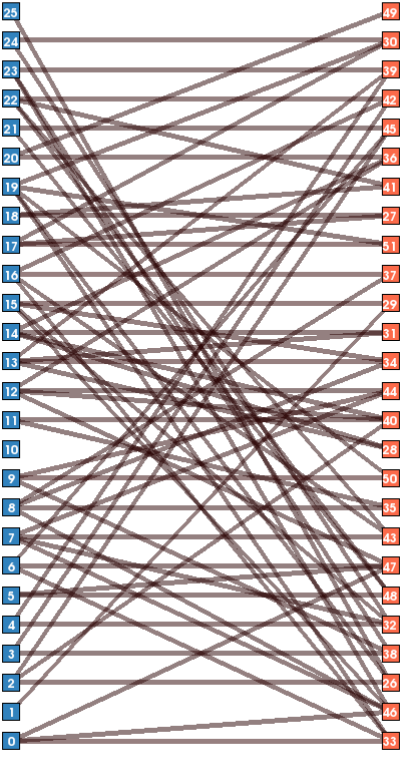
\includegraphics[scale=0.20]{lda_lsa_topic_view}
\end{subfigure}
\begin{subfigure}{.33\textwidth}
  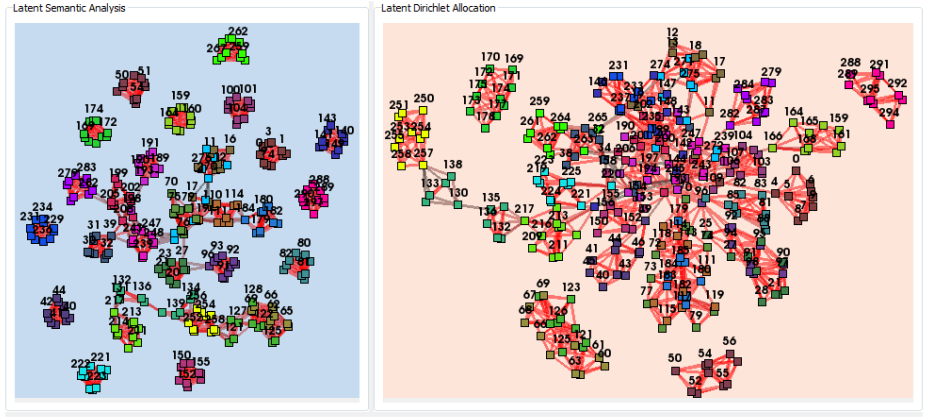
\includegraphics[scale=0.35]{lda_lsa_document_view}
\end{subfigure}
\caption{(Left) Bipartite topic conceptual similarity graph. (Middle, Right) Document relationships formed by LSA and LDA topic modelling methods \label{fig:topic_modelling_comparisons}}
\end{figure}

\renewcommand{\baselinestretch}{2.0}\normalsize
These visualisations might be effective at explaining why a perticular model performs in a certain way at some secondary task, or it might be useful for identifying traits of models that ar valuable for perticular tasks. However, the visualisations don't provide any quantitative insight into how one model may perform when compared to another.

\section{Entity Modeling}
Entity Modelling exists as a small field of study aside from topic modelling and could be regarded as an extention of the NER domain. It relates to the extraction of entity description s, as well as the linking of distinct entities. Many of the challenges in this field stem from the high levels of ambiguity present in natural language. Attempts have been made to utilise Topic Models in the task of entitty resolution as well as forming links and relationships between entities within a document, Whilst semantic resources have been investigated as tools for the automatic tagging of extracted entities.

\subsection{Entity Linking}
Entity linking is the task identifying how entities in a corpus relate to each other, It involves the resolution of entity mentions that refer to the same entity in order to perform optimally.

Topic models have been utilised in the task of entity linking through the application and development of specialised Entity-Topic Models.One such investigation involved finding mentions of concrete entities, such as \('iPod',\, 'Steve Jobs',\) and \(iPhone\) and forming a unifying \('Apple\, Inc'\) topic.~\cite{Han2012-gy} The approach added an additional step to the generative LDA algorithm which sampled topic, and entity assignments for each entity. The focus of the paper utilising the topical context within which each entity was mentioned, to try and resolve entities with multiple mentions through relationships that may form between entities in the model.

The Entity-Topic Models suggested are statistically sound, and perform well in predictive tasks oriented around wikipedia information. The key drawback for this study is the use of short documents to train, test, and evaluate derived models. Models were trained dataset of news articles from the TAC 2009 dataset ~\cite{Macnamee-pd}, which being short in length often benefit the assumption made in the study regarding how entities relate to the topics within the document. For longer texts and perticularly narratives, this assumption is not necessarily valid; wide ranges of topics may be present, with entities only being expressed in the context of some of these topics. The limitation of this entity-topic modelling method could come from the base LDA method. As a bag-of-words approach, 

\subsection{Entity Topic Models}



%
%
% Chapter 3 - New Ideas
%
%
\chapter{New Ideas}
\section{Introduction}
Many different methods of analysis and topic modelling have been considered, with only those specifically discussing the generation of entity-topic models beginning to progress towards meeting the aims that this project has. Of any methods considered, each Entity-Topic Modelling approach had underlying assumptions that rendered them ineffective unless utlised under specific conditions. Additionally, no method directly addressed a need for, or the concept of, a Latent Entity.

The primary contribution of this investigation is a pipeline through which Latent Entity models can be explored. Conceptually, Latent Entity models provide a novel means of summarising, relating, and understanding written narratives. The pipeline propsed utilises a combination of new and existing approaches, with the Latent Entities being extracted using simple clustering methods. As an abstraction of underlying layers of entity topic models, it is necessary to ensure that assumptions made in literature are addressed, else flaws in any developed system ma be further apmplified.

In order to address a fundamental flaw in many aspects of literature on Entity topic models, this investigations proposes the use of a association weighting metric that allows entities to have associations with terms in a document quantified. The Gaussian Entity-Term Matrix outlined in this chapter allows the assumption that entities in a document are equally associated to terms and topics in the same document to be removed.

Evaluating topic modelling methods is a process that requires careful and considerate attention. It has been shown to be possible to evaluate topic models from a variety of perspectives, including the ability to reduce perplexity, as well as their interpretability. As an abstraction from Entity Topic-Models, typical methods for evaluation may not be applicable, alternatives are proposed in this chapter.

It becomes increasingly difficult to visualise and interpret statistical models as their complexity increases, with the meaning of models becoming obsfucated by the variability of data being analysed. Topic models are no exception to the effect that variability has on levels of obsfucation, and as methods increase in complexity, the need for exploratory tools also increases. In addition proposing a pipeline for extracting latent entities, a system for the visualisation and comparison of topic models is proposed.

\section{Gaussian Entity-Term Matrix}

The Gaussian Entity-term matrix (GETM) is a means of segmenting a given document into entities and associated terms. The matrix for a given document consists of strengths of associactions between a entity-word pairing. It functions under an assumption that the more seperation there is between two words in a document, the weaker the association is between those two  words. By modelling documents not as a bag of words, but as sequences it is possible to capture some of the relationships between different words prior to applying additional statistical methods.

Given a set of entities \(\underline{E} = \{\underline{e}_0, ..., \underline{e}_i\}\) where \(\underline{e}_i = \{e_{i,0}, ..., e_{i,m}\}\), and a set of words \(\underline{W}=\{\underline{w}_0, ..., \underline{w}_j\}\), then a matrix \(D\) when indexed by \(i,j\) can be defined as:

\[
  D_{i,j}= \sum^{|\underline{e}_i|}_{m=0}\sum^{|\underline{w}_j|}_{n=0}\sqrt{a\over{\pi}}\cdot e^{-a\cdot(e_{i,m} - w_{j,n})}
\]

\[
  D =
  \bordermatrix{&&e_0 && e_1 &&\hdots && e_i\cr
    w_0 && D_{0,0} && D_{0,1} && \hdots && D_{0,i}\cr
    w_1 && D_{1,0} && D_{1,1} && \hdots && D_{1,i}\cr
    \vdots && \vdots && \vdots && \ddots && \vdots\cr
    w_j && D_{j,0} && D_{j,1} && \hdots && D_{j,i}
  }
\]

This method makes use of the assumption that the more distance there is between two words, or the more words there are seperating two words, the less associated the two words are with each other. There are benefits and downsides to this simplification of the structure of written language. One down side to the assumption made is that, as associations between terms might exactly follow a gaussian distribution, it is possible that the associations between some terms may be exagerated, whilst others are understated. Additionally, the additive approach to handling terms occuring multple times means that there is potentially a need to normalise strengths off associations, this results in additional processing steps that could mitigated by considering alternative methods of handling multiple occurences.


\begin{table}[h!]
  \centering
  \begin{displayquote}
 ``Someone standing outside the Great Hall might well have thought some
sort of explosion had taken place, so loud was the noise that erupted
from the Gryffindor table. Harry, Ron, and Hermione stood up to yell and
cheer as Neville, white with shock, disappeared under a pile of people
hugging him.'' -- J. K. Rowling
    \end{displayquote}
    \begin{tabular}{c | c c c c}
     &Harry&Hermione&Ron&neville\\
      \hline
      loud    & 0.6 & 0.5  & 0.4  & \\
      white   & 0.1 & 0.2  & 0.1  & \\
      shock   & 0.1 & 0.2  & 0.2  & \\
      yell    & 0.2 & 0.1  & 0.3  & \\  
    \end{tabular} 
  \caption{ Example GETM for entities within text \label{fig:getm_example}}
\end{table}

As Figure ~\ref{fig:getm_example} demonstrates, there results in associations between terms that are not necessarily meaningful, the association of Harry to other associations of Harry is not of value, similarly, the association of Harry to words such like 'as' and 'on' is also misleading. As the GETM is only preserving the notion of words having previously held structure and meaning, it is possible to remove perticular parts of speech that don't provide useful insights into the relationships entities have with words. Removing an entity's association to itself is not so straight forward, it requires resolving which mentions refer to which entities, and in cases where entities are either refered to by different names, or two entities share the same name, that is a difficult task. One solution is to ignore entity-entity associations in the GETM, this is perhaps the best approach given the purpose of the GETM. By removing entity-entity associations from the GETM, latent entity models will describe classess of entities, and are less likely to orient themselves around the relationships between entities.

By modelling associations using a Gaussian prior, it is then possible to adjust the hyperparameter \(\alpha\) to increase or decrease the rate at which strengths of association decline as the number of seperating words increase.

It is also possible to remove the gaussian aspect of a GETM, instead utilising different weighting functions. In some texts it might be known that words surrounding entities are associated with strengths following different distributions, thus it is possible to substitute the Gaussian for a more representative prior. 

\subsection{GETM Evaluation}
There is no need for hand crafted methods of evaluating the performance of a GETM, or the effect that a GETM has on the ability for meaningful latent entities to be derived. By fixing all values of the GETM to 1.0 (using a fixed weighting function), an entity can be associated with each term in a given document, this would encode the assumptions made in literature directly into the GETM. The fixed GETM can then be used as a baseline to compare different GETMs, whether that be adjusting parameters in the function, or utilising alternative weighting function.

As a result of GETMs being specifically formed for the task of Latent Entity extraction, it is necessary to evaluate from that perspective, the suitability of the method to other tasks would require more generalised evaluation methods. With the availability of a fixed weighting function when calculating the GETM allows for the comparion of quality between calculated Topic moels and Latent Entities with and without the use of a GETM.

\section{Entity Topic Model}
By using a GETM prior to deriving topic models words are already associated with entities, this makes extending LDA topic models a more simple task. As LDA is a bag-of-words method, each entity and its associated terms within the GETM could be regarded as a distinct document. Using GETMs add an additional set of pre-processing steps to the standard LDA algorithm.

The proportional topic distributions in an Entity Topic Model using the GETM can be calulated by multiplying the strength of association between an entity and a given word, with the word-topic probabilities calculated in an LDA model.
\[
  T_{k,e} = \sum^w \phi_{k,w} \cdot D_{e,w}
\]

Where  \(T_{k,e}\) is the Entity Topic for topic \(k\) and entity \(e\), \(D_{e,w}\) is the strength of assocation between entity \(e\) and word \(w\), and \(\phi_{k,w}\) is the topic-word probability for topic \(k\) and word \(w\).

You may wish to each topic score in an entity topic, bringing values into the \([0,1]\) range. In which case the value for each \(T_{k,e}\) becomes:
\[
  T_{k,e} = {\sum^w {(\phi_{k,w} \cdot D_{e,w})} - max(\underline{T}_e)}\over{ max(\underline{T}_e) - min(\underline{T}_e)}
\]
where \(\underline{T}_e\) is the set of topics for entity \(e\).

\subsection{Evaluating ETMs}

\section{Latent Entities}
A Latent Entity is an abstract statistical model that approximately describes some entities within a corpus. Identifying Latent Entities is possible though clustering entity topic models extracted from a corpus. In the case of k-means clustering, each entity in a GETM matrix is expressed as distributions of entity topics and turned into an Entity-Topic Model. Each Entity-Topic Model can then be clustered in n-dimentional space on topic distributions. The center of each cluster extracted through k-means can then be labelled as a latent entity which abstractly represents entities within that cluster.

As each latent entity remains a probability distribution of entity topics, it is possible to state how similar a given entity is to a latent entity. Each similarity metric of entity to latent entity can then be used to express the entity in terms of similarities to latent entities.

\begin{table}[h!]
  \centering
  \begin{tabular}{*2c}
      \multicolumn{2}{c}{Harry}\\
      Term&Strength\\
      \hline
      Scar&0.1\\
      Magic&0.09\\
      Muggles&0.09\\
      Expelliarmus&0.05
    \end{tabular}              
    \begin{tabular}{*2c}
      \multicolumn{2}{c}{Hermione}\\
      Term&Strength\\
      \hline
      Magic&0.11\\
      Wand&0.09\\
      Superiority&0.04\\
      Unkempt&0.04      
    \end{tabular}
    \begin{tabular}{*2c}
      \multicolumn{2}{c}{Ron}\\
      Term&Strength\\
      \hline
      Drooble&0.07\\
      Magic&0.06\\
      Snigger&0.05\\
      Sherbert&0.03
    \end{tabular}
  \caption{Example entity-term associations between three entities\label{fig:example_entity_term_associations}}
\end{table}

\begin{table}
  \centering
    \begin{tabular}{*4c}
      Topics&Harry&Hermione&Ron\\
      \hline
      Topic 1 & 0.6 & 0.5  & 0.4 \\
      Topic 2 & 0.1 & 0.2  & 0.1 \\
      Topic 3 & 0.1 & 0.2  & 0.2 \\
      Topic 4 & 0.2 & 0.1  & 0.3 \\  
    \end{tabular}
    \vline \,
    \begin{tabular}{*1c}
      \multicolumn{1}{c}{Latent Entity}\\
      \hline
      0.5 \\
      0.13 \\
      0.17\\
      0.2\\
      
      \end{tabular}
  \caption{Example entity-Topic distributions for entities in Table~\ref{fig:example_entity_term_associations} and the associated Latent Entity. \label{fig:example_entity_topic_distribution}}
\end{table}

Given a set of entities (like Harry, Ron, and Hermione), a Latent Entity for this set could be derived by computing the average entity topic model. Conceptually this latent entity could describe entities that can be classified as 'wizards' or 'students'. The exact interpretion of what the latent entity represents is up for debate, in a similar way to how the topic expressed in a topic model is open to interpretation.

Latent Entities in this form could even be used as a means of assisting in the interpretation of large groups of entity topic models. A summary of ETM clusters can be given allowing for higher level overviews of latent structures within a corpus, or elements of a corpus.

\subsection{Application of K-Means}
K-Means clustering is just one approach that can be taken with regards to extracting latent entities from a collection of entity topic models. It is entirely appropriate to utilise other clustering methods, including techniques such as Fuzzy C-Means, Gaussian Mixture Models, or heirarchical style clustering. K-Means as a simple method provides a straightforward approach to finding Latent Entities.

K-Means is a method for minimising variance between clusters and as such can be described as
\[
  \underset{S}{argmin} \sum^{k}_{i=1}\sum^{}_{x\in S_i}||x-\mu||^2
\]
Given this, the equation for determining a set of latent entities for a given collection of entity topic models involves the substitution of the equation for an entity topic model \(T_{k,e}\) into the standard formula for k-means.
\section{Evaluating Latent Entities}
The evaluation of topic models is a challenging task, many techniques commonly used are inherently flawed or difficult to carry out. Many of the flaws present in topic modelling evaluation methods may be made even more pronounced if used to evaluate Entity Topic Models, and Latent. An adaptation of the intruding word test applicable to ETMs proposed here is the intruding Entity Test. Some evaluation metrics are proposed as means of evaluating the quality of latent entities.

\subsection{Intruding Entity}
The intruding entity test involves asking human participants to identify the entity that doesn't belong in a set of entities supposedly represented by a latent entity. The set of entities can be formed by choosing some amount of entities most strongly represente by a Latent Entity, then selcting and adding to the set an entity least likely to be represented by the same latent entity.

Similarly to the intruding word test, the intruding entity test is supposed to performs as a means of evaluating the cohesiveness of the latent entity. Should the set of entities actually be made of those conceptually related, then the odd entity should be identified with a high success rate across all participants.

\begin{figure}[h!]
  \centering
  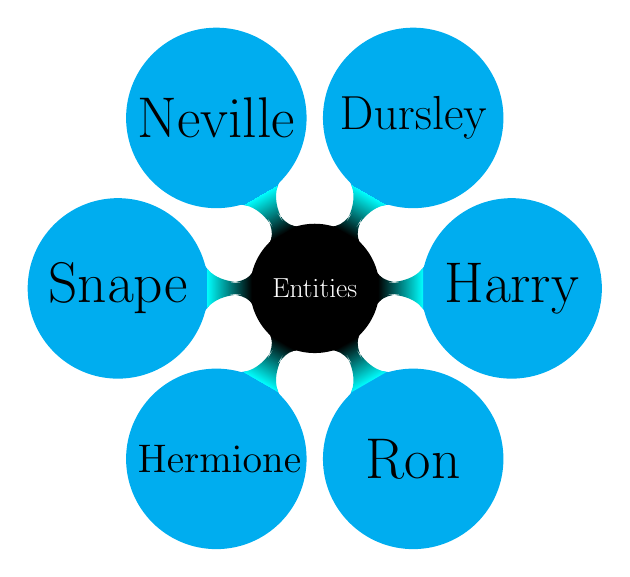
\begin{tikzpicture}
  \path[mindmap,concept color=black,text=black, scale=0.5]
    node[concept,text=white ,scale=0.4, font=\fontsize{28pt}{28pt}\selectfont] {Entities}
    [clockwise from=0]
    child[concept color=cyan] {
      node[concept,  font=\fontsize{20pt}{20pt}\selectfont]
      {Harry}
    }  
    child[concept color=cyan] {
      node[concept,font=\fontsize{20pt}{20pt}\selectfont]
      {Ron}
    }
    child[concept color=cyan] {
      node[concept, font=\fontsize{15pt}{18pt}\selectfont]
      {Hermione}
    }
    child[concept color=cyan] {
      node[concept, font=\fontsize{20pt}{20pt}\selectfont]
      {Snape}
    }
    child[concept color=cyan] {
      node[concept, font=\fontsize{20pt}{20pt}\selectfont]
      {Neville}
    }
    child[concept color=cyan] {
      node[concept, font=\fontsize{18pt}{20pt}\selectfont]
      {Dursley}
    };
  \end{tikzpicture}\\
Select the entity that does not belong the the set: \underline{\quad \quad \quad \quad \quad \quad}
  \caption{Example Set of Entities for the Intruding Entity Test.\label{fig:intruding_entity}}
\end{figure}

In Figure~\ref{fig:intruding_entity} you can see an example of how the test may look, the names of entities being presented in some format, with participants requested to select the entity that does not belong. There are a range of influencing factors that could invalidate the results of any test of this format, most notable of which is the familiarity of the participants to the reference material. In cases where individuals are unfamiliar with the narratives from which entities are drawn from, then there would be increased difficulty when selecting the conceptually unrelated entity.

Admittedly, there is a range of investigations that can be carried out to evaluate the efficacy of this method of evaluation. It might be necessary to provide participants with additional information about the set in order to allow them to make informed decisions. As the entities within the set are them selves represented by topic models, it is possible to then provide information regarding the words associated with those entities that resulted in the set of entities represented by the calculated Latent Entity.

\begin{figure}
  \centering
  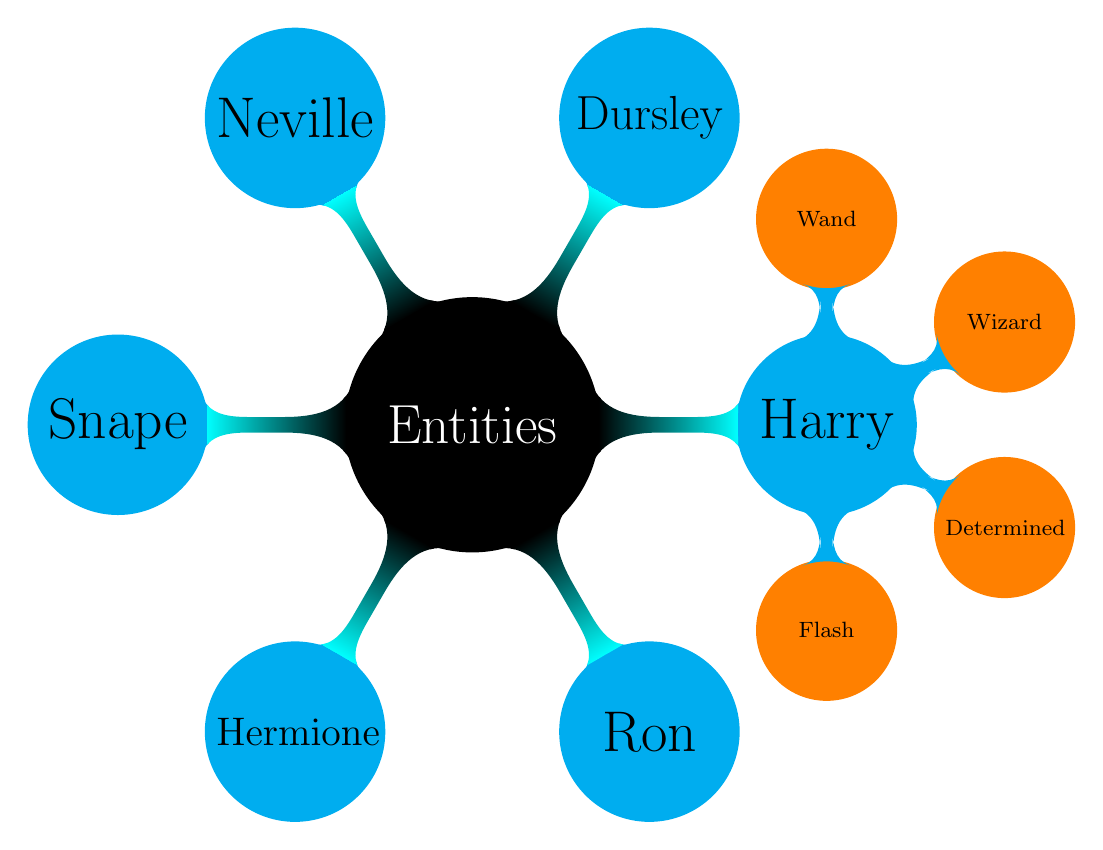
\begin{tikzpicture}
      \path[mindmap,concept color=black,text=black, scale=0.9]
    node[concept,text=white ,scale=0.8, font=\fontsize{28pt}{28pt}\selectfont] {Entities}
    [clockwise from=0]
    child[concept color=cyan] {
      node[concept,  font=\fontsize{20pt}{20pt}\selectfont]
      {Harry}
      [clockwise from=90]
      child { node[concept, color=orange, text=black] {Wand} }
      child { node[concept, color=orange, text=black] {Wizard} }
      child { node[concept, color=orange, text=black] {Determined} }
      child { node[concept, color=orange, text=black] {Flash} }
    }  
    child[concept color=cyan] {
      node[concept,font=\fontsize{20pt}{20pt}\selectfont]
      {Ron}
    }
    child[concept color=cyan] {
      node[concept, font=\fontsize{15pt}{18pt}\selectfont]
      {Hermione}
    }
    child[concept color=cyan] {
      node[concept, font=\fontsize{20pt}{20pt}\selectfont]
      {Snape}
    }
    child[concept color=cyan] {
      node[concept, font=\fontsize{20pt}{20pt}\selectfont]
      {Neville}
    }
    child[concept color=cyan] {
      node[concept, font=\fontsize{18pt}{20pt}\selectfont]
      {Dursley}
    };
\end{tikzpicture}
  \caption{Example Set of Entities with Set of Associated Terms.\label{fig:intruding_entitiy_terms}}
\end{figure}

For participants that are unfamiliar with the matrial from which the entities in the set are from, presenting the terms most strongly associated with the entities might resolve the impact that this could have on their ability to select the correct entitiy. Of course, with the addition of more information the question becomes more complex to answer, there becomes more factors to consider when determining which entity is the unrelated one.


\subsection{Evaluating Consistency}
The consistency of the proposed method for calculating latent entities can be determined by comparing the results of the process for two corpora of different documents onthe same subject. The assumptions for this method of evaluation is that the contents of books on the same subject are likely to be similar, whilst this may not be true for narratives, factual books on the same subject should hold true.

The consistency check can be used to evaluate different stages of the analysis pipeline. The GETM aspect of the system is a prime candidate for this form of evaluation. Similarly, entities within the GETM should be associated with the same or synonymous terms if assumptions regarding the similarity of two copora are true.

By using copora that are known to be similar in content would remove the perhaps dangerous assumption. However, the corpora are not the same, and thus there still remains the chance that any difference in compared models would be a result of the differences in documents between each corpora.

\subsubsection{Latent Entity Consistency}
For latent entities, it is necessary to consider entities that are present in both corpora that have been clustered differently, and the number of entities absent from one or the other document.

Considering common entities, consistency is calculated using the number of consistencies or true positive (TP), and inconsistencies or false positive (FP) entity pairings within each latent entity clusters. TP is the number of entity pairings in a latent entity cluster present in both sets of latent entities, FP is the opposite of that, the number of entity pairings within clusters not the same across both sets of latent entities.

Where $N$ is the number of Latent entities clusters, and $n_i$ is the number of entities within the latent entity cluster indexed by $i$, consistency is defined as:
\[
  Consistency = \frac{TP - FP}{\sum^{N}_{i=1}{n_i\choose2}}
\]

The defined consistency metric ranges from $-1.0$ to $1.0$. Values approaching $1.0$ mean the two sets are increasingly correllated.

\begin{table}[h!]
  \centering
  \begin{tabular}{c | c | c}
    Cluster 1 & Cluster 2 & Cluster 3 \\
    \hline
    a & 1 & x \\
    b & 2 & y \\
    c & 3 & z \\
    d & 4 & w \\
  \end{tabular}
  \quad
  \begin{tabular}{c | c | c}
    Cluster 1 & Cluster 2 & Cluster 3 \\
    \hline
    a & d & x \\
    1 & 2 & b \\
    c & y & 3 \\
    2 & 4 & w \\
  \end{tabular}
  \caption{Left \& Right: Entities Within Clusters Behind Latent Entities.\label{tab:latent_entity_clusters}}
\end{table}

An example of the consistencies and inconsistencies between two sets of latent entities seen in Table~\ref{tab:latent_entity_clusters} can be seen in Table~\ref{tab:latent_entity_consistencies}. With the total number of pairings, $\sum^{N}_{i=1}{n_i\choose2} = 16$, a $TP=4$ and $FP=12$ the consistency of these two sets of latent entities is $\frac{4-12}{16} = -0.5$. A negative value implies the latent entiteis are entirely different compositions, and are very inconsistent.

\begin{table}
  \centering
  \begin{tabular}{c | c c c c}
    Constencies
    & (a, c) 
    & (1, 2) 
    & (x, w) 
    & (4, 2)
    \\
    \hline
    Inconsistencies
         & (a, 1) 
         & (a, 2) 
         & (c, 1)                      
         & (c, 2)
         \\
         & (d, 2) 
         & (d, 4) 
         & (y, 2) 
         & (y, 4)
         \\
         & (x, b) 
         & (x, 3) 
         & (w, b) 
         & (w, 3) 
  \end{tabular}
  \caption{Consistencies and Inconstencies Between Clusters Forming Latent Entities\label{tab:latent_entity_consistencies}}
\end{table}


\subsubsection{GETM Consistency}
Calculating the consistency of the GETM method requires numerically evaluating similarity of terms associated with common entities between two GETMs. Additionally, the entities not common to both need to be incorporated into the calculation.




\section{Analysis Pipeline}
The Analysis Pipeline is a series of steps necessary for the task of extracting Latent Entities from a Corpus. Each step can be viewed as a transformation which can be applied to the results of the previous step.

The pipeline is essential to the implementation of a system which can be used to extract Latent Entity information. Without consideration of what the steps would be, the value of any developed system could be severely diminished.

Starting with raw documents, the start of the process is the tokenization of each document in the corpus. The extraction of POS tag information and Entities within the corpus can be carried out in parallel, it is necessary that both tasks are performed prior to the calculation of the Gaussian Entity-Term Matrix. From the GETM, Entity-Topics and subsequently Latent Entities can be extracted.

\begin{figure}[h!]

  \centering
  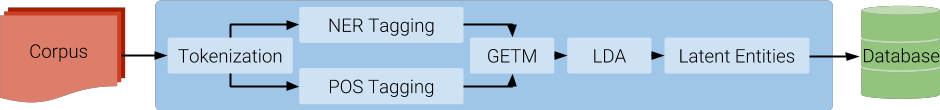
\includegraphics[scale=0.445]{pipeline_diagram_bold}
  \caption{Analysis Pipeline for the Extraction of Latent Entity Information.\label{fig:pipeline_diagram}}
\end{figure}

\section{Topic Model Explorer}

As machine representations of words most probably related topically, topic models are not always easy to interpret. Presenting only a set of terms within a topic might not provide the best insight into what that topic represents in a corpus. The challenges of interpretation are further compounded as layers of abstractions are added to a topic model. Entity Topic Models and subsequently Latent Entities would be easier to intepret when presented alongside other derived models. As such, a topic model explorer is proposed as a tool allowing the comparison and exploration of topic models, entity topic models, and latent entities.

Humans often try to understand a topic by applying a single word or small phrase as a title of any given topic. Latent Entities are abstractions of multiple Entitiy Topic Models, with each entity topic model being varying distributions of topics and words. In order to accomodate for the human need to label models, the Topic Model Explorer can accomodate for this by demonstrating how different clusters of entity topic models are similar, extracting words most siginificant across members of the cluster.

As well as allowing comparisons of entity topic models, by allowing the explorer to accomodate for the comparison of other levels of topic model extractions, it can allow individuals to evaluate the quality of each model used to describe a corpus.

\subsection{Interface}
The interface for the Topic Model Explorer is a key aspect in allowing individuals to understand the machine models extracted from a corpus.

\subsection{Visualisations}

%
%
%
%
%
\chapter{Implementation}
\section{Introduction}
For an investigation to be carried out into the possibility and efficacy of latent entities, it is necessary to begin with the implmentation of a framework through which a study can be carried out. As such implementation for this project involves the development of 3 key elements:

\renewcommand{\baselinestretch}{0.5}\normalsize
\begin{itemize}
\item Analysis Toolkit
\item Web Server Architecture
\item Latent Entity Explorer
\end{itemize}
\renewcommand{\baselinestretch}{2.0}\normalsize
The Analysis Toolkit involves the derivation and implementation of methods necessary to process and analyse corpora. Web Server Architecture involves the design and implementation of a database, Server, and API capable of allowing access to processed data and results from analysis. The Latent Entity Explorer entails the creation of a set of visualisations and tools allowing for the exploration of Entity-Topic models and Latent Entities.

Once the base framework is in place, implementation turned towards the task of evaluating the proposed process for extracting latent entities, as well as refining implementations.

\section{Architecture Overview}
The system principally follows a standard 3 layer approach to web-server architecture, requiring a database (DB), web server and API, and a client application. This implementation uses PostgreSQL as its DB of choice, as well as following RESTful practices in the API design. The web server is implemented in python, with a DB repository layer accompanying the server and API implementation. The client application (Latent Entity Explorer) is implemented using TypeScript and the Angular 5 framework.

\begin{figure}[h!]
  \centering
  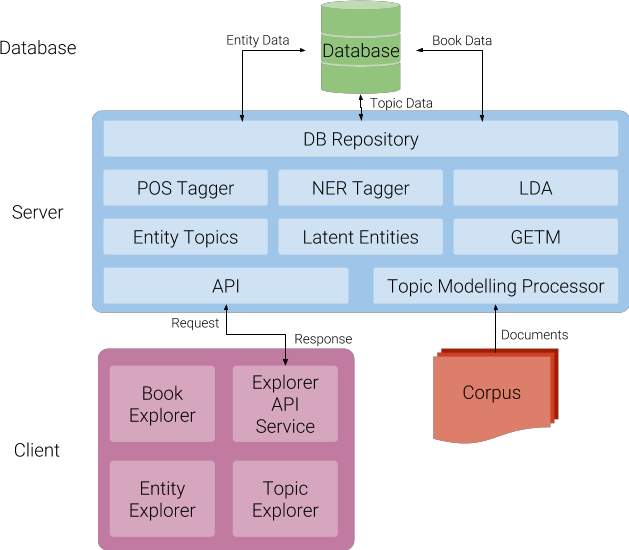
\includegraphics[scale=0.55]{architecture_diagram}
%   \begin{tikzpicture}>=latex,shorten >=2pt,shorten <=2pt,shape aspect=1

%   \matrix[matrix of nodes, row sep=5ex, column sep=1em] (mx) {
%     Database:& |[cy]| Database \\
    
%     Server:&
%     |[rs=3]|
%     \nodepart{one}DB Repository
%     \nodepart{two}Application Logic
%     \nodepart{three} REST API &
%     |[rs=3]|
%     \nodepart{one} Repository Layer
%     \nodepart{two} System Logic Layer
%     \nodepart{three} API Layer
%     \\
%     Client:& |[rs=3]|
%     \nodepart{one}DB Repository
%     \nodepart{two}Application Logic
%     \nodepart{three} REST API &
%     |[rs=3]|
%     \nodepart{one} Service Layer
%     \nodepart{two} Component Layer
%     \nodepart{three} User Interface Layer
%     \\
%   };
%   \node[ou=(mx-2-2)] (server) {};
%   \node[ou=(mx-3-2)] (client) {};
%   {[->]
%   \draw (server)edge(mx-1-2) (mx-1-2)edge(server) (client)edge(server) (server)edge(client);
%   }
% \end{tikzpicture}
  
  \caption{Architecture overview of the Latent Entity Model Analysis and Exploration System. \label{fig:architeture_overview}}
\end{figure}


Alongside the server is a set of Analysis Tools that were developed as distinct methods with utility in their own right.

\subsection{API}
The focus of the API is to allow clients to interact with data resulting from the analysis pipeline. Data to be made available will primarily consist of book meta-data, and extracted information relating to topic models, entity topic models, and Latent Entities.

Given the defined purpose of the API, and the process through which narratives can be analysed, the design of endpoints is a relatively straightforward task. The API will consist of a series of GET request endpoints for book data, as well as a small set of endpoints allowing additional narratives to be added to the system and analysed.

A Subset of the endpoints in the api for requesting data from the system can be seen in Table~\ref{tab:api_endpoints}, each of which are GET requests. There are additional endpoints that allow for other aspects of collected and extracted data to be requested, as well as POST endpoints that allow or additional documents to be added to the system.

\begin{table}[h!]
\centering
\begin{tabular}{r | l}
  Endpoint&URI\\
  \hline
  Book Titles        & /api/ books \\
  Book Topics        & /api/books/\guillemotleft book title\guillemotright/topics \\
  Book Entities      & /api/books/\guillemotleft book title\guillemotright/entities \\
  Book Topics terms  & /api/topics/\guillemotleft topic id\guillemotright \\
  Entity Topics      & /api/books/\guillemotleft book title\guillemotright/entities/\guillemotleft Entity Name\guillemotright/topics \\
  Entity Topic Terms & /api/books/\guillemotleft book title\guillemotright/entities/\guillemotleft Entity Name\guillemotright/topics/\guillemotleft topic id \guillemotright \\
  Latent Entities    & /api/latent\\
  Latent Entity Topics & /api/latent/\guillemotleft Latent Entity ID\guillemotright
    \end{tabular}
  \caption{ Selection of API Endpoints.\label{tab:api_endpoints}}
Text between guillemots represent variables of the URI.
\end{table}

From Table~\ref{tab:api_endpoints} it is clear how most of the endpoints are oriented around a book title, however, it would not make sense to follow this structure for latent entities. As latent entities are representative of a collection of entities, they are not part of any singular book, and thus are not accessed in the same means as other aspects of the API.

\subsection{Database} The database is implemented using PostgreSQL, primarily due to familiarity that is held with the DB and library interfaces for various languages (including Python and JavaScript). Additionally, PostgreSQL is an Open Source database implementation, meaning that it is a morally justifiable choice of software.

The database is a key element of the overall system, it is required to provide a persistent means of storing and accessing large amounts of data. There can be vast amounts of data extracted from a corpus, and the amount of time that a process can take to perform the task would mean days are spent waiting for a request to be completed should extracted data not be stored upon completion of analysis.

\subsubsection{DB Structure}
The Database design was to be oriented around two key concepts: Book Entities, and Topics. Building the DB around these concepts allows for some reflective structure to be maintained between the way that data is stored, and the way that users can access it through the API. The benefit to this is to a developer implementing aspects of software between the database and API, resulting in easier implementation of system logic and analysis tools that access data through the repository layer. Figure ~\ref{fig:db_erd} shows the relational structure of tables in the database.

\begin{figure}[h!]
  \centering
  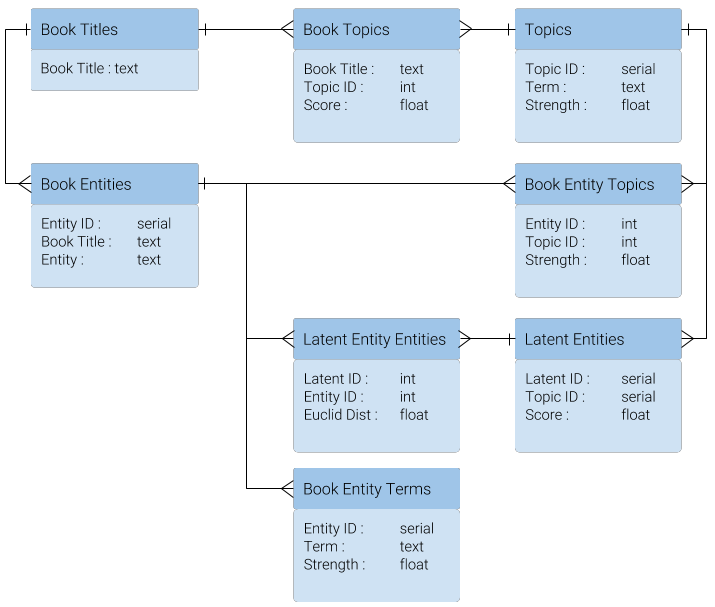
\includegraphics[scale=0.5]{db_erd}
  \caption{Entity Relationship Diagram Showing the Structure of the System's Database.\label{fig:db_erd}}
\end{figure}

A significant table to the system is the 'Book Entity Terms' table, which is a relational database form of a GETM extracted from a corpus. Principally, the table allows for the calculation of Entity Topic Models and Latent Entities to be carried out a later time, whilst also allowing an investigation into how the GETM influences resulting Models.

The tables, 'Latent Entities' and 'Latent Entity Entities' are an important pair for the system, they handle the numerical descriptions of Topics forming each Latent Entity, as well as how each entity in the corpus influenced the structure of each latent Entity.

\subsection{Server}
The Server for this system holds both the API and various distinct processing units forming the system logic. Implemented in Python, the server intergrates well with existing libraries for processing natural language and interacting with databases, it allows for the fast development of a REST API, as well as having a convenient PostgreSQL Library.

The top layer of the server, as shown in Figure~\ref{fig:architeture_overview} is the repository layer. The Repository layer handles all interactions with the database. Below the Repository layer are two layers of processing units with each providing different elements of functionality to the system, from performing POS tagging, to clustering Entity Topic Models.

Below the system logic layers sit two potential interface elements. The first, being the API allows web clients to query and interface with the system, the second is a command line interface element that allows processing of corpora to be initiated and carried out locally within the server.

\subsubsection{Repository}
Using a repository style pattern for separating the responsibility of interfacing with the database means that a clear structure for inserting, updating, and retrieving data can be defined. In this system, the repository is utilised by both the API and the various processing units and system logic shown in Figure~\ref{fig:architeture_overview}.

\subsubsection{System Logic Layers}
The collection of system logic layers consist primarily of methods for carrying out distinct tasks. Many of which satisfy requirements placed on the system by the proposed pipline diagrammed in Figure~\ref{fig:pipeline_diagram}.

Much of the functionality made available to the system is made available at the command line, locally on the server. This is due to the computationally intensive nature of the system, many of the tasks can take days of processing if given a large corpora. A corpus of 7 books could take approximately 3 hours to calculate a GETM for.

Each element of the System Logic Layer explored in further detail when discussing the NLP Toolkit.

\section{NLP Toolkit}
As any investigation involving the use of data in any form does, pre-processing was carried out on the collections of documents intending to be analysed. As this investigation aims to also serve as a tool from which multiple corpora can be analysed, the pre-processing steps taken need to be reproducible. The NLP Toolkit developed for this system is essentially a collection of tools that allow each document in the corpus to be pre-processed ready for the extraction of topic models and latent entities. A somewhat functional approach was used, with each method applying some transformation to a single document, or a corpus as a whole. The Analysis Pipeline defined in chapter 3 involves tasks starting with the Tokenization of plain text, and ending with the use of clustering methods to extract Latent Entities.

The toolkit can be viewed as a combination of both simple and complex NLP methods, that allow basic NLP tasks like tokenization and POS tagging to be carried out, as well as more complex GETM and topic modelling techniques.

\subsection{General NLP}
Tokenizing, POS Taggin, NER, an other pre-processing tasks are required as defined in the proposed analysis pipeline. A collection of NLP Utilities allow these tasks to be carried out within the system being developed. Table~\ref{tab:nlp_utilities} shows some of the methods developed, as well as their purpose within the system

\begin{table}[h!]
  \begin{tabular}{c | p{0.6\linewidth} }
    Method & Purpose\\
    \hline
    $sent\_tokenize(document)$ & Returns an array of string tokens representing sentences within the provided document  \\
    $word\_tokenize(sent\_tokens)$& Returns a mapping of sentence tokens to arrays of word tokens \\
    $tag\_document(word\_tokens)$ & Returns an array of POS tag sequences for each sentence of word tokens\\
    $tag\_entities(word\_tokes)$ & Returns an array of tagged entity tuples using NER tagger\\
    $cherry\_entity\_tuples(entities)$ & Returns a mapping of entity names from set of entity tuples\\
  \end{tabular}
  \caption{NLP Ultity Methods\label{tab:nlp_utilities}}
\end{table}

\subsubsection{POS Tagging}
A Viterbi Decoded Hidden-Markov Model was implemented to perform the task of POS Tagging. The Viterbi tagger acted as a baseline from which existing taggers could be compared against. Most notably, the NLTK POS Tagger was selected as a potential POS tagging tool, this was a result of how easy the tagger is to use, and how simply it integrates with other libraries.

A dynamic programming algorithm, the Viterbi algorithm provides a comparatively computationally efficient way of decoding Markov processes, or in this case, find the most probable sequence of POS tags for a given sequence of words. This implementation followed the process described by Algorithm~\ref{alg:viterbi_decoder}

\renewcommand{\baselinestretch}{1.0}\normalsize
\begin{algorithm}[H]
  \caption{Viterbi Decoding Algorithm\label{alg:viterbi_decoder}}
  \begin{algorithmic}
   
    \STATE let $O$ be the sequence of observations.
    \STATE let $S$ be the set of possible states 
    \STATE let $V$ be the sequence of sets of state probabilities 
    \STATE let $P$ be the POS-tagged sequence of word tokenized sentence tokens
    \STATE let $G$ be the Gaussian Entity-Term Matrix.
    \STATE
    \STATE $S\gets sentTokenize(document)$
    \FOR{$S_s \in S$}
      \STATE $W_s \gets wordTokenize(S_s)$
      \ENDFOR
      \STATE 
    \STATE $E \gets extractEntities(W)$
    \STATE $P \gets posTag(W)$
    \STATE $G \gets calculateGETM(E, G)$
    \STATE
    \RETURN $E, P, G$
    
  \end{algorithmic}
\end{algorithm}
\renewcommand{\baselinestretch}{2.0}\normalsize


\subsection{Gaussian Entity-Term Matrix}


\subsubsection{Algorithm}


\subsubsection{GETM Objects}



\section{Corpus Pre-Processing}

Corpus Pre-Processign involves applying a set of transformations necessary to begin the analysis and creation of descriptive models. It is assumed that the corpus provided to the system will contain only the text that is to be processed. In many documents there is additional preamble, publishing information, and other elements that can be considered 'noise'. This system will not concern itself with the removal of noise within the corpus.

Tokenization is the first transformation to be applied to the corpus. NLTK provides a suite of tools capable of kickstarting any NLP project, including methods for tokenizing documents. With the option to tokenize a document into sentences, and then words, there are different approaches that can be taken to tokenization. This project uses the default tokenization methods which use XXXXXXXXXXXXXXXXXXXXXXXXXXXXXXXXX. It is important that the documents are tokenized into sentences, and then each sentence is tokenized into words, as this structure allows for more effective POS tagging.

Once each document in the corpus has sentences and words tokenized, the next stage in the processes is the application of POS tagging methods to determine the gramatical structure of each sentence. A Viterbi Decoded Hidden Markov Model (HMM) POS tagger was implemented in python, utilising the NLP tookit developed for this project. POS Tagging this document means that it is possible to apply filters to the corpus before deriving topic models from the GETM. By removing certain words tagged as certain POS (like determiners, or prepositions) it is possible to derive topics using only descriptive words, which may provide more cohesive and interpretable models.

Figure~\ref{fig:document_preprocess} shows the process taken by the system to apply pre-processing methods to an individual document in the corpus. beginning with tokenization, and ending with the calculation of a GETM for that document. Figure~\ref{fig:corpus_preprocess} denotes the process of assimilating a collection of documents into the system.

\renewcommand{\baselinestretch}{1.0}\normalsize
\begin{algorithm}[H]
  \caption{Document Pre-processing steps\label{fig:document_preprocess}}
  \begin{algorithmic}
   
    \STATE let $S$ be the sequence of sentence tokens, where $S_s$ is a sentence token.
    \STATE let $W$ be the sequence of word tokenized sentence tokens, where $W_s$ is a set of word tokens for sentence token $S_s$.
    \STATE let $E$ be the set of entities where $E_e \in W$.
    \STATE let $P$ be the POS-tagged sequence of word tokenized sentence tokens
    \STATE let $G$ be the Gaussian Entity-Term Matrix.
    \STATE
    \STATE $S\gets sentTokenize(document)$
    \FOR{$S_s \in S$}
      \STATE $W_s \gets wordTokenize(S_s)$
      \ENDFOR
      \STATE 
    \STATE $E \gets extractEntities(W)$
    \STATE $P \gets posTag(W)$
    \STATE $G \gets calculateGETM(E, G)$
    \STATE
    \RETURN $E, P, G$
    
  \end{algorithmic}
\end{algorithm}
\renewcommand{\baselinestretch}{2.0}\normalsize

\renewcommand{\baselinestretch}{1.0}\normalsize
\begin{algorithm}[H]
  \caption{Corpus Pre-processing steps\label{fig:corpus_preprocess}}
  \begin{algorithmic}
    \STATE let $T$ be the set of document titles
    \FOR{$t \in T$}
      \STATE $D \gets openDocument(T)$
      $E$
    \ENDFOR
  \end{algorithmic}
\end{algorithm}
\renewcommand{\baselinestretch}{2.0}\normalsize

\section{Entity-Topic Model}

\subsection{Algorithm}

\section{Latent Entity Clustering }

\section{Latent Entity Explorer}


%
%
%
%
%
\chapter{Results and Evaluation}
\section{Introduction}

\section{POS Tagger}

\subsection{Results}


\section{Gaussian Entity-Term Matrix}
Whilst the Gaussian Entity-Term Matrix (GETM) was defined only as a means overcome particular prior assumptions in literature it is necessary to evaluate the quality of associations formed within the matrix. Should the quality of underlying associations be poor, then the Entity-Topic models and Latent Entity Models will never be able to accurately capture entity structures within narratives.

\subsection{Experiment Setup}

\subsection{Results}

\section{Entity Topic-Models}
The use of a GETM was proposed as a means removing an assumption made in literature regarding the relationships which entities have with the topics within a document. It is therefor necessary to evaluate how the adapted approach performs.

\subsection{Experiment Setup}

\subsection{Results}

\section{Latent Entities}

%
%
%
%
%
\chapter{Conclusion}
\section{Introduction}

\renewcommand{\baselinestretch}{1.0}\normalsize
\bibliographystyle{unsrt}
\bibliography{./biblio}
\end{document}
